\chapter{Project Planning Schedule}
\makeatletter\@mkboth{}{Appendix}\makeatother
\label{appen:PP}

\begin{table}[h]
\centering
\begin{tabularx}{\textwidth}{|c|X|c|}
\hline
\textbf{Week} & \textbf{Work Planned to Start} & \textbf{GanttChart Ref.} \\
\hline
1 & Conduct Detailed Research on BMS Topology & Research \\
\hline
2 & Draft Abstract Report & Abstract \\
\hline
3 & Initiate System Design Process & Design \\
\hline
4 & Conduct Extensive Datasheet Consultations & Datasheet \\
\hline
5 & Execute Circuit Designs & Circuit \\
\hline
6 & Source Components \& Initiate Ordering Process & Components \\
\hline
7 & Engage in Printed Circuit Board Design Process & PCB Design \\
\hline
8 & Review \& Revise Circuit and PCB Designs & Review \\
\hline
9 & Place Order for Printed Circuit Board & Order PCB \\
\hline
10 & Solder Components \& Conduct Module Debugging & Debugging \\
\hline
11 & Design Reporting \& System Analysis Testing & Reporting \\
\hline
12 & Evaluation \& Conclusion Reporting & Evaluation \\
\hline
\end{tabularx}
\end{table}
     \begin{figure}[!htb]
     \centering
     	\fbox{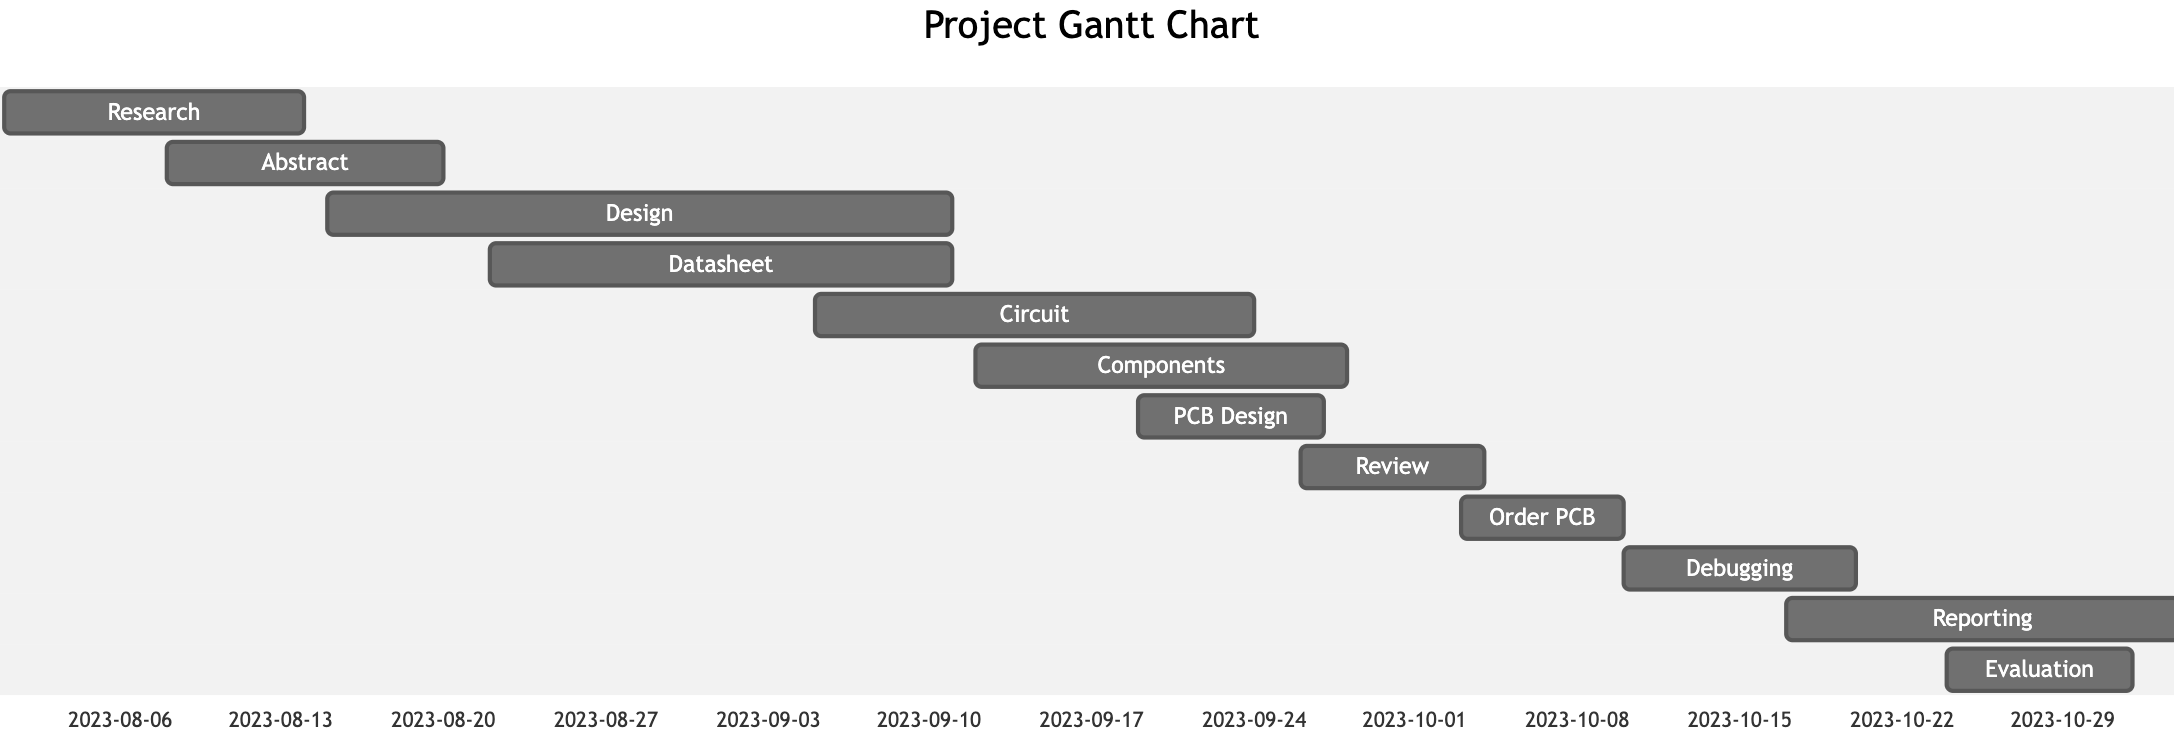
\includegraphics[width=1\linewidth]{./Figures/GanttChart.png}}
	\label{fig:ProjectShed}
	\end{figure}